%=========================================================================
% (c) 2014, 2015 Josef Lusticky

\section{Egress traffic processing}\label{sec:linux-egress}
The previous sections described how the frame reception works and the way they are passed when
the routing subsystem decides to forward them.
After the routing decision is made and the {\it{skb}} is passed to the {\it{ip\_finish\_output()}} function,
it is further passed back to the link layer part of the stack.
This part of the Linux networking also provides interface to the device drivers
and handles traffic control~\cite{understanding-internals}.

In reference to the egress traffic processing, there are two important functions in this part of the stack -
{\it{dev\_queue\_xmit()}} and {\it{dev\_hard\_start\_xmit()}}.
The {\it{ip\_finish\_output()}} function of the IPv4 stack passes the outgoing {\it{skb}}
to the {\it{dev\_queue\_xmit()}} function, which determines whether the device is queueless of queueful~\cite{understanding-internals}.
If the device is queueless, such as Loopback or Virtual interface, then the {\it{skb}} is passed to
{\it{dev\_hard\_start\_xmit()}} directly without any traffic control mechanism involved.
The {\it{dev\_hard\_start\_xmit()}} function further prepares the {\it{skb}} for transmission
and passes it to the transmission function of the device driver,
which instructs the device to transmit the frame on the wire~\cite{understanding-internals}.

If the device is queueful, such as almost any hardware network adapter, {\it{dev\_queue\_xmit()}}
executes the traffic control first~\cite{understanding-internals}.
The traffic control implemented in the Linux kernel uses algorithms known as queuing disciplines
(often abbreviated as qdisc)
to arrange the frames in the most efficient order for transmission~\cite{understanding-internals}.
Figure~\ref{fig:linux-egress-packet} shows the above described part of the stack.
\begin{figure}
	\centering
	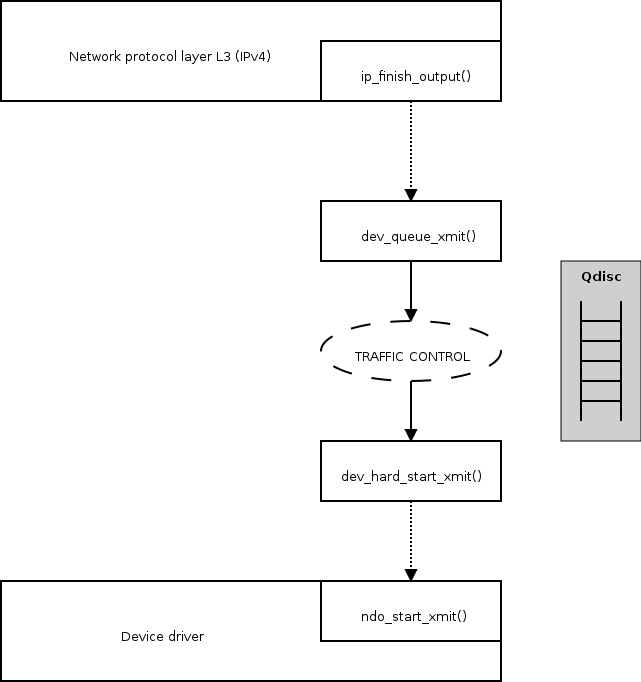
\includegraphics[width=10cm,keepaspectratio]{fig/kernel-layer2-flow.png}
	\caption{Egress packet processing}
	\label{fig:linux-egress-packet}
	\bigskip
\end{figure}

The default queuing discipline for every network device where
no custom configuration has been applied is fifo\_fast~\cite{linux-kernel-networking}.
As the name suggests, the fifo\_fast is a classless First In First Out discipline,
that is, the first packet to get in, is going to be the first to be sent~\cite{tcpip-in-linux}.

After the packet has been selected for transmission by the traffic control, it is passed to the
{\it{ndo\_start\_xmit()}} function, which is implemented by the device driver~\cite{kernel-source}.
The packet is inserted to the hardware transmit queue by the driver.

Linux kernel supports multiple queuing disciplines, that can be configured by the {\it{tc}} utility.
A more detailed discussion of the traffic control and its queuing disciplines is outside the scope of this thesis.
Currently two qdiscs are optimised for multiqueue devices.
The first is the default pfifo\_fast qdisc.
This qdisc supports one qdisc per hardware queue.
The mq (multiqueue) qdisc is a dummy scheduler.
It is used by default for multiqueue devices instead of the regular pfifo\_fast qdisc,
but can also be attached manually to restore multiqueue behaviour
after attaching a non-multiqueue (shared) qdisc~\cite{kernel-doc-multiqueue}.

%%%

The networking subsystem has been assigned two different softirqs -
NET\_RX\_SOFTIRQ handles incoming traffic and NET\_TX\_SOFTIRQ handles outgoing traffic.
Because different instances of the same softirq handler can run concurrently on different CPUs,
networking code is both low latency and scalable~\cite{understanding-internals}.

\subsection{Transmit offloads}
Most of the adapters that support receive checksum offload,
also support its counter-part option to offload transmission (Tx) checksums.
Tx checksum offload calculates TCP/UDP and
IP checksums of the packets in the hardware before they are transmitted on the wire.

%TODO Scatter-gather feature allows the network adapter to read from and write to
%non-contiguous areas during direct memory access (DMA)~\cite{linux-kernel-networking}.

A counter-part of LRO is TCP Segmentation Offload (TSO).
With a TSO-capable adapter, the kernel can prepare much larger packets (e.g. 64KB)
for outgoing data and the adapter will re-segment the data into smaller packets according to the MTU~\cite{jls2009-gro}.
TSO is well supported in Linux -
for systems which are engaged mainly in sending of data, it is sufficient to make 10Gb line-rate at full speed~\cite{jls2009-gro}.
TSO reduces the necessary CPU load, bus overhead, and cache impact to send a series of packets,
but it still does not require the adapter to actually know
anything about specific TCP connections -
the kernel still has to deal with the TCP states and ACKs~\cite{linux-and-tcp-offload-engines}.

The TCP Segmentation Offload is designed to work with TCP exclusively.
To mitigate this issue, the Generic Segmentation Offload (GSO) was implemented, which is not limited to TCP.
Performance improves even if the feature is emulated in the driver~\cite{jls2009-gro}.
Figure~\ref{fig:linux-tx-offloads} shows comparision of egress processing
with and without the above described offload mechanisms.
\begin{figure}
	\centering
	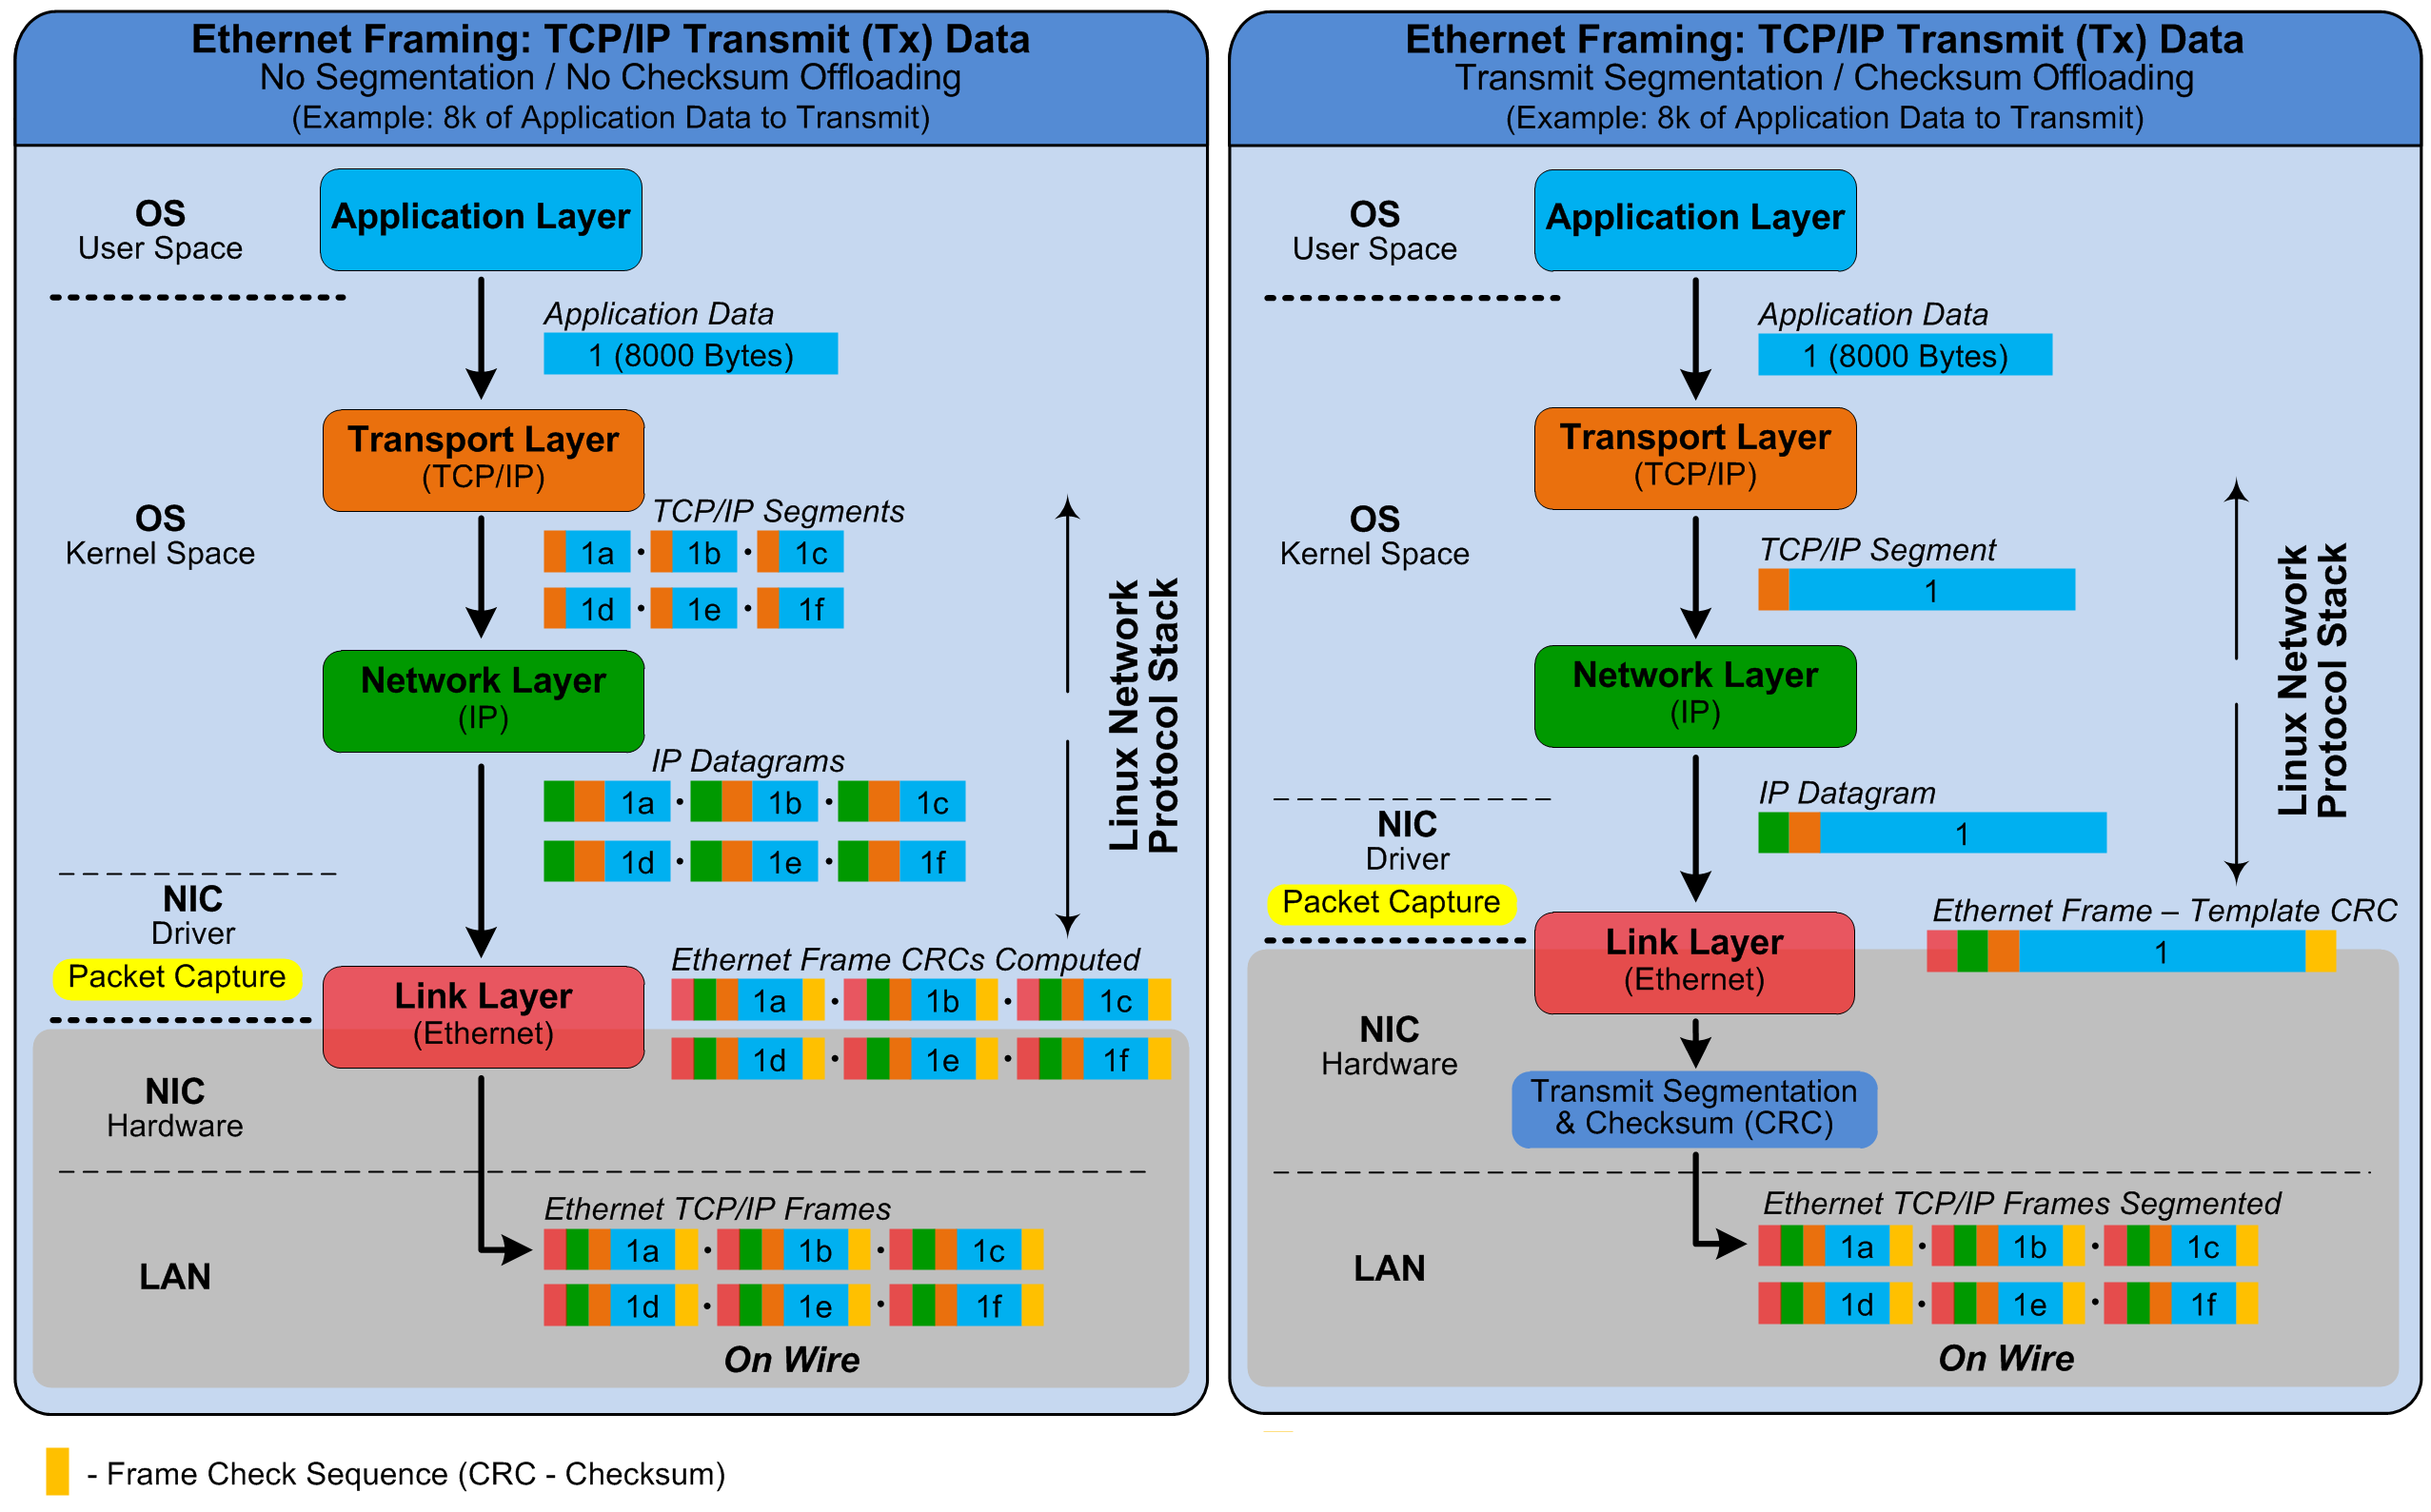
\includegraphics[width=15cm,keepaspectratio]{fig/tx-offloads.png}
	\caption{Transmit offloads (source:~\cite{nst-offloads})}
	\label{fig:linux-tx-offloads}
	\bigskip
\end{figure}

%Large Receive Offload (LRO) packets are dropped in forwarding.
%Forwarding a large SKB, which was
%built by LRO, is not acceptable because it will be larger than the outgoing MTU.
%Therefore, when LRO is enabled the
%SKB is freed and the method returns NET\_RX\_DROP.
%Generic Receive Offload (GRO) design included forwarding
%ability, but LRO did not~\cite{linux-kernel-networking}.
